\documentclass[10pt]{article}

%%%%%%%%%%%%%%%%%%%%%%%%%%%%%%%%%%%%%%%%%%%%%%%%%%%%%%%%%%%%%%%%%%%%%%%
% ICCAD'26 (paper #571) -- Author Round-1 Response
% Word budget: ~2000 words. Reviewer color tags: R1=571A, R2=571B,
% R3=571C, R4=571D.
%%%%%%%%%%%%%%%%%%%%%%%%%%%%%%%%%%%%%%%%%%%%%%%%%%%%%%%%%%%%%%%%%%%%%%%

\usepackage[margin=0.7in]{geometry}
\usepackage[dvipsnames]{xcolor}
\usepackage{graphicx}
\usepackage{enumitem}
\usepackage{amsmath}
\usepackage{titlesec}
\usepackage{subcaption}
\graphicspath{{ICCADRebuttal/Pics/}{Pics/}}

\setlist{nosep,leftmargin=1.2em}
\titlespacing*{\section}{0pt}{4pt}{2pt}
\titlespacing*{\paragraph}{0pt}{3pt}{6pt}
\titleformat{\section}{\normalfont\large\bfseries}{\thesection}{0.5em}{}

% Reviewer color tags
\definecolor{c1}{HTML}{1F77B4}
\definecolor{c2}{HTML}{2CA02C}
\definecolor{c3}{HTML}{D62728}
\definecolor{c4}{HTML}{9467BD}
\newcommand{\R}[1]{\textbf{R#1}}
\newcommand{\Ra}{\textbf{\textcolor{c1}{R1}}}
\newcommand{\Rb}{\textbf{\textcolor{c2}{R2}}}
\newcommand{\Rc}{\textbf{\textcolor{c3}{R3}}}
\newcommand{\Rd}{\textbf{\textcolor{c4}{R4}}}
\newcommand{\ans}{\textbf{$\Rightarrow$~}}

\pagestyle{empty}
\setlength{\parindent}{0pt}
\setlength{\parskip}{3pt}

\begin{document}

\begin{center}
{\large\bfseries Rebuttal Response Round 1--- Paper \#571}\\[2pt]
{\small ``Automated Architecture-Aware Generation of Large Integer Multipliers on FPGAs''}\\[2pt]
{\footnotesize Reviewer tags: \Ra\,(571A)\quad \Rb\,(571B)\quad \Rc\,(571C)\quad \Rd\,(571D)}
\end{center}

\vspace{2pt}
We thank all reviewers.
We are encouraged that the work is seen as addressing ``a genuine and practically important gap'' that prior flows leave open (\Rd), as ``The promised open-source release would be a useful artifact'' (\Rc), with a ``relevant IR optimizer and good results compared to related work``(\Ra).
Below we group shared concerns first, then reviewer-specific points.
We commit to every textual change mentioned.

%%%%%%%%%%%%%%%%%%%%%%%%%%%%%%%%%%%%%%%%%%%%%%%%%%%%%%%%%%%%%%%%%%%%
\section*{1. Novelty: the contribution is not just in the tiler but the overall architecture-aware automation \hfill {\normalsize(\Rb,\,\Rc,\,\Rd)}}

\Rc\ suggests framing the contribution ``primarily as architecture-aware automation'' rather than as multiple distinct algorithmic advances; \Rb\ asks what the novelty is.
\textbf{We agree with \Rc's framing and will adopt it.}
The novelty is \emph{not} a new tiler in isolation; it is that every step is shaped with the DSP architecture in mind to jointly maximize frequency \emph{and} minimize scarce DSP usage, which no prior automated large-multiplier flow does:
\begin{itemize}
\item \textbf{Square Base Multiplier} scaling a square base turns the very few rectangular Karatsuba alignments (e.g.\ $26{\times}17\Rightarrow442k$) into dense ones ($44{\times}44\Rightarrow44k$), which is what \emph{enables} deep Karatsuba which allows for DSP savings.
\item \textbf{Separation of term generation from DSP mapping}, enabling DSP cascade-aware grouping (0-bit or 17-bit shifts), arithmetic rewrites (1-bit multiplications $\to$ AND, and $P1+(P2{\ll}n)\to\{P2,P1\}$ to zero-cost concatenate instead of accumulation).
These saves expensive operations with cheaper ones, and saves LUTs by integerated post-adder in the DSP cascade instead of separate logic.
\item \textbf{Pipeline-schedule-aware reduction} This is integrated into all the parts from the combinational logic to the internal DSP registers to the final output registers to allow automatically pipelining at the right points to break the combinational ceiling and reach high frequency.
This is not just a ``deep pipelining'' step; it is a per-component scheduling that allows pipelining to be effective without excessive latency or resource overhead.
This also enables the segmentation step that allows trading off latency for frequency.
\end{itemize}
We suggest the measurements show this is more than ``pure engineering'' (\Rb): the same arithmetic, mapped without architecture awareness (the HLS baseline in Table~2), runs at 298\,MHz with \emph{more} LUTs and DSPs than our 458--478\,MHz designs.

%%%%%%%%%%%%%%%%%%%%%%%%%%%%%%%%%%%%%%%%%%%%%%%%%%%%%%%%%%%%%%%%%%%%
\section*{2. What drives the gains? (and the iso-pipeline ablation) \hfill {\normalsize(\Rc\,Q1,\,\Rd)}}

\Rd\ and \Rc\ ask whether the frequency gain comes from the arithmetic mapping or merely from deeper pipelining, and request an iso-pipeline ablation.
\textbf{Deep pipelining is necessary but not sufficient}, and existing results separate the two effects:

\begin{enumerate}
\item \textbf{Base multiplier, single level, no deep tiling (Fig.~6, Table~1).}
Before any hierarchical pipelining, our 77-bit base already beats the AMD IP: higher frequency, 2 fewer DSPs.
This isolates \emph{mapping} from \emph{depth}.
\item \textbf{Resources, not just frequency.}
Segment pipelining cannot reduce DSP count; only the decomposition/mapping can.
At 1024-bit, other works use 17--45\% more DSPs than our proposed approach --- a result pipelining alone cannot produce.
\item \textbf{Per-component attribution:}
\begin{itemize}
\item \emph{Base selection} sets the DSP floor and the achievable frequency (scaling a slow/wasteful base cannot recover either).
\item \emph{Hierarchical decomposition} controls how deeply Karatsuba removes multipliers (Table~2: more Karatsuba levels $\to$ fewer DSPs).
\item \emph{Cascade-aware mapping} cuts LUTs used for logic (\S3.2) and raises frequency.
\item \emph{Optimizer rewrites} trade eligible expensive operations to cheaper ones, such as replacing 1-bit multiplications with AND gates or using zero-cost concatenations instead of accumulation saving resources and critical path delay.
\item \emph{Segmentation} (Table~3) choosing the combination of segment size and pipeline depth allows trading off latency for frequency.
\end{itemize}
\item \textbf{The requested cross-mapping ablation is approximated by the HLS row.}
``IMpress mapping + our pipelining'' is not runnable by us --- IMpress is HLS, and we cannot re-pipeline a competitor's closed flow at any granularity without their generator.
The honest iso-tool point already in the paper is the HLS baseline: same arithmetic left to the tool, far worse frequency \emph{and} more resources.
We will state this limitation explicitly and add the per-component breakdown above as a short ablation paragraph.
\end{enumerate}
\textbf{On the ``4--5$\times$ pipeline depth''} (\Rc,\,\Rd): high frequency requires depth, but Table~3 shows depth is a \emph{tunable knob}, not a fixed cost --- a 256-bit segment cuts latency 100$\to$58 cycles while still beating prior work on frequency.
We will frame this tradeoff more explicitly.

%%%%%%%%%%%%%%%%%%%%%%%%%%%%%%%%%%%%%%%%%%%%%%%%%%%%%%%%%%%%%%%%%%%%
\section*{3. Single-vendor / cross-platform generality \hfill {\normalsize(\Ra,\,\Rc,\,\Rd)}}

Three reviewers ask about generality of our approach beyond AMD UltraScale+.
\ans \textbf{The flow is vendor-agnostic by construction; only the leaf instantiation templates are architecture-specific.}
The Versal/DSP58 result (Table~2) is the evidence: moving from a $27{\times}18$ to a $27{\times}24$ primitive, the tiler, hierarchy generator, untimed IR, software simulation, scheduling, and RTL/testbench generation are all \emph{reused unchanged} --- only the DSP instantiation template and board constraints differ.
Porting to Intel/Altera Stratix/Agilex therefore requires authoring the DSP instantiation template, project/reporting templates, and constraint files, not rewriting the algorithms (\Rb's ``what is assumed'').
We will state this porting checklist explicitly and soften ``broadly applicable'' to ``architecture-parameterized, demonstrated on two AMD DSP generations''

On \Ra's Altera specifics:
\begin{itemize}
\item \emph{Square primitives}. Stratix 10 has a $27{\times}27$ hard multiplier, so the primitive is already square allowing immediate Karatsuba alignment. The only difference between the flow for AMD and Intel is only the hardware primitive instantiation template; the rest of the flow is unchanged.
\item \emph{Hard fixed-point cores.} Stratix 10 has hard fixed-point cores that can be used for multiplication, but they are not relevant to wide integer multiplication. 

\end{itemize}

%%%%%%%%%%%%%%%%%%%%%%%%%%%%%%%%%%%%%%%%%%%%%%%%%%%%%%%%%%%%%%%%%%%%
\section*{4. Architectural difference vs.\ the AMD IP \hfill {\normalsize(\Ra)}}

\Ra\ asks how our design is architecturally different from the AMD IP (not just in final resources).
\ans \textbf{We tried to conclude the decomposition of the 64-bit IP from the device view.}
It instantiates 16 DSPs with 15 PCOUT$\to$PCIN cascade connections, i.e.\ \emph{fully cascaded design}, which means that all inter-tile shifts are 0 or 17.
This means that the IP caps each DSP to $\le17{\times}17$ (we confirmed $17{\times}17$, $17{\times}13$, $17{\times}18$ tiles via reporting non-fixed port widths in the dsp block through Tcl console), implying a $(17,17,17,13)$ decomposition.
Replicating it reproduces its results to within $\approx$100~LUTs / 50~FFs (shift logic);
With this decomposition, the base multiplier IP is wasteful, as it does not use the full $27{\times}18$ capability of the DSPs.
If we had chosen schoolbook decomposition, we would have used only 11 DSPs instead of 16 with the decomposition shown in Fig.~\ref{fig:ours64}.
When scaling to 1024-bit, this would still be using more DSPs than our 43-bit base, but it will be much more optimal than using the direct IP. 
If we stick to the same decomposition, we can use Karatsuba to save 4 of the 16 DSPs, but it will be wasteful especially when scaling to larger sizes, and this is shown in Fig.7.
This is precisely the architecture-aware advantage.
We will add this analysis and the figures.

% Optional figures (include if response format permits images).
\begin{figure}[h]
\centering
\begin{subfigure}{0.32\linewidth}\centering
  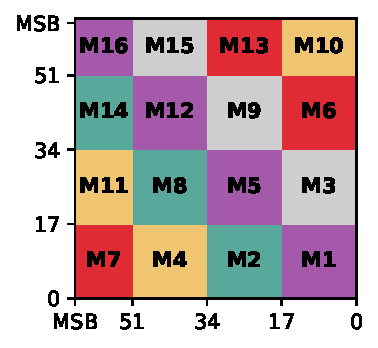
\includegraphics[width=\linewidth]{Tiling_RectFig64x64.pdf}
  \caption{IP's $(17,17,17,13)$ decomposition (16 DSPs).}
  \label{fig:ip}
\end{subfigure}\hfill
\begin{subfigure}{0.32\linewidth}\centering
  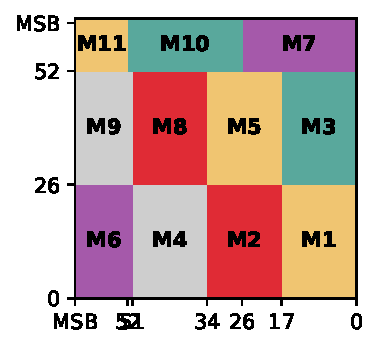
\includegraphics[width=\linewidth]{Tiling_RectFig64x64_bettersb.pdf}
  \caption{Our Schoolbook mapping (11 DSPs).}
  \label{fig:ours64}
\end{subfigure}\hfill
\begin{subfigure}{0.32\linewidth}\centering
  
\includegraphics[width=\linewidth]{Tiling_RectFig78x78.pdf}
  \caption{Our 78-bit base (14 DSPs).}
  \label{fig:ours78}
\end{subfigure}
\caption{(Fig.~A) AMD IP vs.\ our architecture-aware mappings.}
\end{figure}

%%%%%%%%%%%%%%%%%%%%%%%%%%%%%%%%%%%%%%%%%%%%%%%%%%%%%%%%%%%%%%%%%%%%
\section*{5. FFs and the normalized-area metric \hfill {\normalsize(\Rc)}}

\Rc\ notes $A_{\text{norm}}=\#\text{LUTs}+126\cdot\#\text{DSPs}$ excludes FFs while our designs use 207K--274K FFs.
\ans \textbf{We just used the exact metric of the prior work we compare to}.
FFs are excluded in all the works we denote as N/A 
Anyways, in these devices FFs are the most abundant, rarely the binding resource, whereas DSPs are scarce.
Our design philosophy also provide a tradeoff knob to reduce FFs at the cost of frequency (Table~3), so including FFs in the metric would shift the tradeoff curve
We agree the asymmetry should be visible and will (i) add an FF column for our designs, (ii) report the prior works' FFs as N/A only because \emph{they do not report them} (\Rc\ Q on N/A), and (iii) add one sentence noting that an FF-inclusive metric would shift the tradeoff but not the DSP-and-frequency advantage, which is the scarce-resource axis.

%%%%%%%%%%%%%%%%%%%%%%%%%%%%%%%%%%%%%%%%%%%%%%%%%%%%%%%%%%%%%%%%%%%%
\section*{6. Table~1 ``LUT inversion'' at 78-bit \hfill {\normalsize(\Rd)}}

\Rd\ asks why 78-bit one-group (537 LUTs) exceeds multi-group (429), contradicting ``one-group uses fewer LUTs,'' and whether counts are post-synthesis with SRL inference.
\ans \textbf{All results reported in the paper are post place and route, and LUTs used in the one-group strategy are Shift-Register LUTs, not logic LUTs.}
The exact count is as following:
The one-group strategy uses 0 logic LUTs while the multi-group strategy uses 62 and 239 logic LUTs for 44-bit and 78-bit respectively.
\textbf{We will split the LUT column into logic-LUTs and SRL-LUTs in Table~1} to make this unambiguous.


%%%%%%%%%%%%%%%%%%%%%%%%%%%%%%%%%%%%%%%%%%%%%%%%%%%%%%%%%%%%%%%%%%%%
\section*{7. Missing comparisons and the \S3.2 vs.\ Table~2 numbers \hfill {\normalsize(\Rc\,Q2,\,\Rd)}}

\textbf{ILP [17] and rectangular-Karatsuba [16]} (\Rc\ Q2/comment~2): the ILP is the \emph{predecessor} of beam-search, which we already report and beat, thus beat the ILP.
The rectangular-Karatsuba work targets a different regime: its largest reported case is $112{\times}120$, and it has no hierarchical decomposition, so it cannot scale to the 1024-bit-and-up ``large integer'' regime we target (their ``large'' means $>64$-bit).
We will add this explanation in \S5 with this explicit justification.

\textbf{OpenNTT row} (\Rd): NTT is a different algorithmic class with a different latency regime (689 cycles); we include it only for context.
We  completed the fields available from their paper and clearly label it as a non-tiling reference rather than a comparison.

\textbf{Reconciling \S3.2 (464/507/516) with Table~2 (810)} (\Rc\ comment~3): these report \emph{different filling strategies}.
The 464/507/516 are DSP counts for only remainder-filling parts denoting different strategies (cascade-compatible vs.\ greedy vs.\ non-cascade). 
Table~2 reports fully-implemented 1024-bit lowest-DSP configuration not just the remainder-filling strips.

%%%%%%%%%%%%%%%%%%%%%%%%%%%%%%%%%%%%%%%%%%%%%%%%%%%%%%%%%%%%%%%%%%%%
\section*{8. Headline percentages \hfill {\normalsize(\Rc)}}

\Rc\ is correct.
\ans The abstract/caption figures are all vs.\ IMpress2 ( what we believe to be the strongest prior approach); \S4.1 is the per-baseline detail.
We also interchangeably used  ``17\% fewer DSPs (ours)'' with ``17\% more DSPs (theirs)''.
\textbf{We will make every percentage consistent, state the baseline inline, and correct the direction of the DSP comparison.}

%%%%%%%%%%%%%%%%%%%%%%%%%%%%%%%%%%%%%%%%%%%%%%%%%%%%%%%%%%%%%%%%%%%%
\section*{9. Remaining points \hfill {\normalsize(\Ra,\,\Rb)}}

\textbf{Experimental setup} (\Ra): EPYC~7763 (64C), 512\,GB RAM, Ubuntu~20.04, Vivado~2022.1, AMD Alveo U280; all results are post-place-and-route.
We will add this to the evaluation section.

\textbf{Why not leave it to HLS / native tools?} (\Rb): because they underperform on this problem; our own HLS baseline (Table~2) runs at 298\,MHz with more LUTs and DSPs, since the tools do not exploit cascade paths, asymmetric ports, or per-DSP pipeline depth for wide structured arithmetic.

\textbf{ML design-space-exploration work} (\Rb): TODO
\medskip
We believe these clarifications and additions (per-component ablation, FF column, logic/SRL LUT split, IP architectural analysis with figures, explicit ILP/Kumm/OpenNTT justification, generality/porting checklist, corrected percentages, and full setup) directly address every concern.
We thank the reviewers for their feedback and for helping us clarify the presentation and strengthen the paper.

\end{document}
